\documentclass{article}%
\usepackage[T1]{fontenc}%
\usepackage[utf8]{inputenc}%
\usepackage{lmodern}%
\usepackage{textcomp}%
\usepackage{lastpage}%
\usepackage[head=40pt,margin=0.5in,bottom=0.6in]{geometry}%
\usepackage{graphicx}%
%
\title{\textbf{Denuncian pago incompleto del salario con fórmula semanal}}%
\author{ANA DÍAZ}%
\date{18/10/2018}%
%
\begin{document}%
\normalsize%
\maketitle%
\textbf{URL: }%
http://www.el{-}nacional.com/noticias/economia/denuncian{-}pago{-}incompleto{-}del{-}salario{-}con{-}formula{-}semanal\_256241\newline%
%
\textbf{Periodico: }%
EN, %
ID: %
256241, %
Seccion: %
Economía\newline%
%
\textbf{Palabras Claves: }%
Economía\newline%
%
\textbf{Derecho: }%
2.3%
, Otros Derechos: %
NO\_TIENE%
, Sub Derechos: %
2.3.4%
\newline%
%
\textbf{EP: }%
SI\newline%
\newline%
%
\textbf{\textit{Trabajadores del sector público protestaron en el centro de Caracas en una marcha conjunta, bloqueada por guardias nacionales}}%
\newline%
\newline%
%
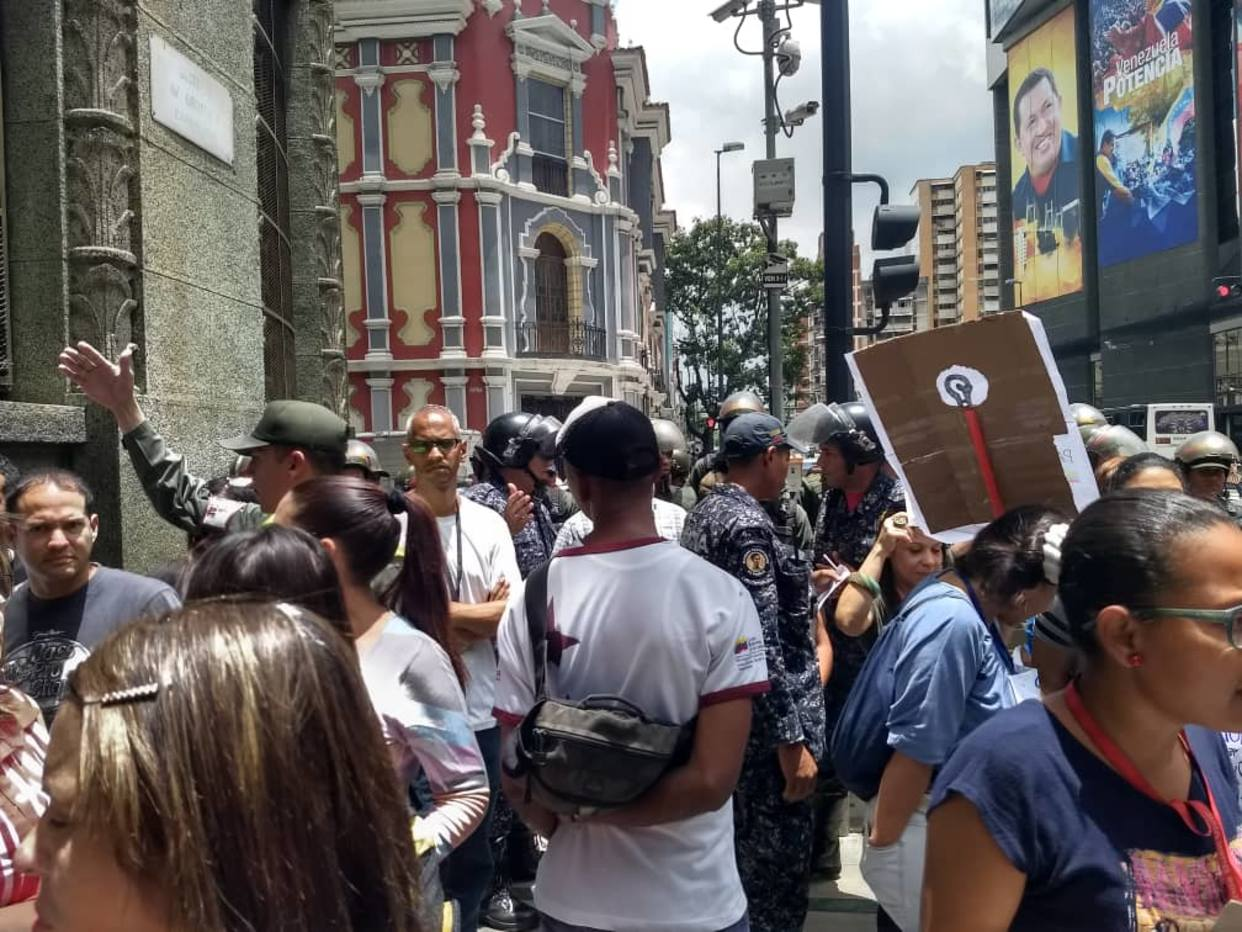
\includegraphics[width=300px]{158.jpg}%
\newline%
%
Las protestas diarias contra la decisión del gobierno de Nicolás Maduro, que desmejoró los tabuladores de sueldos y otros derechos laborales, continuaron ayer en Caracas. La decisión de dirigentes sindicales y de trabajadores, simpatizantes y no simpatizantes del oficialismo, de emprender acciones conjuntas se concretó en~la Plaza~de~la Moneda~del Banco Central de Venezuela.%
\newline%
%
“En esta acción no hay distingo ideológico porque el gobierno irrespeta los derechos de todos los trabajadores con su política de achatar las tablas salariales y eliminar o desmejorar primas y beneficios de la contratación colectiva”, afirmó Pablo Zambrano, directivo del ~sindicato de la salud.%
\newline%
%
Denunció que el~~Ejecutivo cancela~incompleto el sueldo de los empleados públicos con la nueva idea del pago semanal, sobre todo, porque la hiperinflación abatió el poder de compra del salario mínimo de 1.800 bolívares soberanos al mes vigente del 1º de septiembre.%
\newline%
%
El lunes, sindicatos y gremios del sector público decidieron unirse en un comité para defender tabuladores y contratos colectivos irrespetados con las actas{-}convenio suscritas entre el gobierno y dirigentes sindicales afectos, que desmejoran o eliminan beneficios.%
\newline%
%
La semana pasada firmaron las actas{-}convenio de Petróleos de Venezuela, las empresas básicas de Guayana y el Metro de Caracas, mientras que ayer en la tarde se negociaba el de~la Cantv.%
\newline%
%
Reinaldo Díaz, del sindicato de trabajadores eléctricos, alertó que hace 64 días fue suspendida la negociación del contrato colectivo del sector. “Los trabajadores rechazan la sustitución de la convención ~por un acta{-}convenio”, dijo.%
\newline%
%
Marlene Sifontes, del sindicato del Instituto Nacional de Parques, indicó que a los jubilados de Inparques les eliminaron el pago del bono alimentación, establecido en el contrato colectivo, y la asignación de una caja CLAP mensual. “Ese pago semanal del sueldo es un fraude laboral”, sostuvo.%
\newline%
%
Destacó que la reconversión monetaria y la igualación de los sueldos con la imposición de un salario mínimo deprecian las prestaciones sociales. “Ningún empleado quiere jubilarse con unas prestaciones de 4.000 bolívares soberanos por trabajar 30 años, y que no alcanzan ni para un mercado”.%
\newline%
%
Con la consigna de “Presidente Maduro respete los derechos laborales”, trabajadores, dirigentes sindicales y jubilados de la salud, eléctricos, educación, Cancillería, Inparques, Asamblea Nacional, Instituto Nacional de Deportes y empresas de Guayana, entre otros, salieron a la calle desde la plaza del BCV.%
\newline%
%
Los manifestantes, sin embargo, no pudieron llegar a la avenida Urdaneta, a pocas cuadras de Miraflores, porque un piquete antimotín de guardias nacionales se los impidió.%
\newline%
%
\end{document}